\documentclass[a4paper]{proc}

\usepackage{amsmath}
\usepackage{amsfonts}
\usepackage{amssymb}
\usepackage{graphicx}
\usepackage{subcaption}
\usepackage{caption}

\DeclareMathOperator{\expectation}{E}

\newcommand{\euler}{\mathrm{e}}
\newcommand{\diff}{\mathrm{d}}
\newcommand{\T}{^\textup{T}}
\newcommand{\vect}[1]{\mathbf{#1}}
\newcommand{\vectGreek}[1]{\boldsymbol{#1}}
\newcommand{\matr}[1]{\mathsf{#1}}

\begin{document}
\section{Beta prior, binomial likelihood}
\subsection{Method}
Suppose a parameter $\theta$ has a prior distribution such that
\begin{equation}
\theta\sim\textup{Beta}(1,1)
\end{equation}
and that a random variable $X$ is distributed such that
\begin{equation}
X|\theta\sim\textup{Bin}(12,\theta) \ .
\end{equation}
Then after observing $X=2$, the posterior distribution is given as
\begin{equation}
(\theta|X=2)\sim\textup{Beta}(3,11) \ .
\end{equation}
ABC was used to sample the posterior distribution where the algorithm is as followed:
\begin{itemize}
  \item Sample $\theta$ from the uniform distribution
  \item Sample $X|\theta$ from the likelihood
  \item If the sampled $X|\theta$ is equal to 2, accept $\theta$, otherwise reject.
\end{itemize}

\subsection{Results}
10,000 posterior samples were drawn from the ABC algorithm. These were compared with the true posterior distribution, as shown in Figure \ref{binomial}, using the $\chi^2$ goodness of fit test.  By repeating the experiment 50 times, the mean and standard deviation $p$-value for the $\chi^2$ test was found to be $(50\pm30)\%$. This is very strong evidence that the ABC posterior samples do estimate the posterior distribution well.

The mean and standard deviation number of rejected samples per accepted sample was estimated to $(10\pm10)$.

\begin{figure}
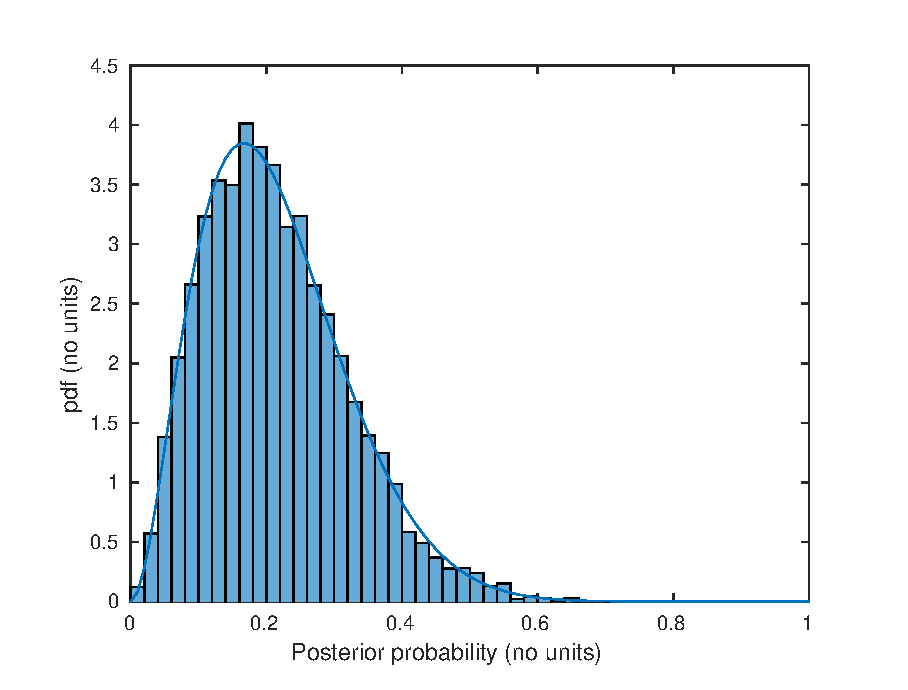
\includegraphics[width=0.5\textwidth]{binomial_ABC0528.eps}
\caption{Histogram of 10,000 posterior samples of $\textup{Beta}(3,11)$ using ABC. The curve shows the exact posterior distribution function. The $p$-value for the $\chi^2$ goodness of fit test in this example was $5\%$ to one significant figure.}
\label{binomial}
\end{figure}

\section{Normal-Gamma prior, Normal likelihood}


\end{document}